\documentclass{article}
\usepackage[utf8]{inputenc}

\usepackage{hyperref}
\usepackage{pgfgantt}
\usepackage{biblatex}
\usepackage{placeins}
\usepackage{geometry}[margin=1in]
\title{Judicial Review}
\author{ Taylor Herald : herald.r@wustl.edu, 451027\\
            Christabel Wayllace : cwayllace@wustl.edu, 460591\\
            Adam Kern : adam.kern@wustl.edu, 441588
}
\date{October 2018}
\hypersetup{
    colorlinks=true,
    linkcolor=blue,
    citecolor=blue,
    urlcolor=blue
}
\bibliography{Proposal-Bibliography}

% \renewcommand{\section}{\FloatBarrier\section}

\begin{document}
\maketitle

\section{Introduction}
The Supreme Court of the United States is one of the most powerful institutions in America; its role in arbitrating disagreements at the highest level allows it to influence policy and daily American life in incredibly concrete ways.  Famous cases such as Brown v. Board of Education and Roe v. Wade decide which children can go to which schools \cite{oyez-brown}, and a woman's right to an abortion \cite{oyez-roe}.  Gideon v Wainwright gave Americans their right to legal representation \cite{oyez-gideon}, and Citizens United v. Federal Election Committee gave corporations the right to give unlimited amounts of money to political elections \cite{oyez-fec}.  These are just a few of the hundreds of cases the Supreme Court has decided on over the years, shaping America with every ruling.\\

Despite this, the Supreme Court remains an unknown part of the American political system.  According to a 2015 Pew Research Center survey, only 34\% of respondents knew who the Chief Justice of the Supreme Court was \cite{pew-scotus-awareness}.  Even optimistic research shows that, in 2005, only 60.5\% of respondents knew that Supreme Court members serve a life term, and only 56.8\% knew that Supreme Court justices serve a life term \cite{gibson-survey}.  In short, the American people are woefully uneducated and misinformed about the role and function of the Supreme Court.\\

With our visualization, we hope to provide a medium through which everyday people --- that may or may not keep up with or understand the Supreme Court --- can gain insight into how the Supreme Court has evolved over the years as well as how it has influenced (and has been influenced by) the American people. The source code of the visualization can be found \href{https://github.com/therald/Judicial-Review.git}{here}.\\

\section{Project Objectives}
The project should support our main objective: provide insight into the evolution of the Supreme Court and its influence on American society. In order to do that, we propose the following sub-objectives:
\begin{itemize}
    \item Show how the political ideology of the Supreme Court justices (liberal vs. conservative) affected the court’s decisions over time. Specifically, we want to show how individual justices’ ideologies changed during their tenure on the Court, as well as how the Court's decisions move ideologically.
    \item Show the Court’s focus and the change and evolution of American society over time by visualizing information about unconstitutional rulings by issue area.
    \item Show how the Court’s and American society’s viewpoints on various issues changed over time by analyzing the court cases that altered precedence in a given area.
\end{itemize}

\section{Data}
The main source of information comes from the Supreme Court Database~\url{http://scdb.wustl.edu/} which provides both modern and legacy data in two versions: (1) Case Centered Data and (2) Justice Centered Data.\\

Additionally, we are also pondering the use of the dataset used in~\cite{fowler:2007} and~\cite{fowler:2008}.

\section{Data Processing}
Data processing for us will most likely come in the form of web scraping. This is due to the fact that although the data is given to us in a .csv format, values for a majority of the parameters are mapped to strings and these mappings are just displayed in the documentation. So, these mappings will be scraped into their own .csv files for the parameters that we choose to dive into. That aside, the data is formatted well in such a way that we should not need to do much more than that.\\

Additionally, we may have to generate new datasets by joining data from the Supreme Court Database with other datasets found online, or compiled by hand, that help to add information to our visualizations.

\section{Visualization Design}
Before coming together to formalize our designs, each group member created a number of sketches for the visualizations.  Included below are a few of them:
\subsection{Option 1}
\begin{figure}[h!]
    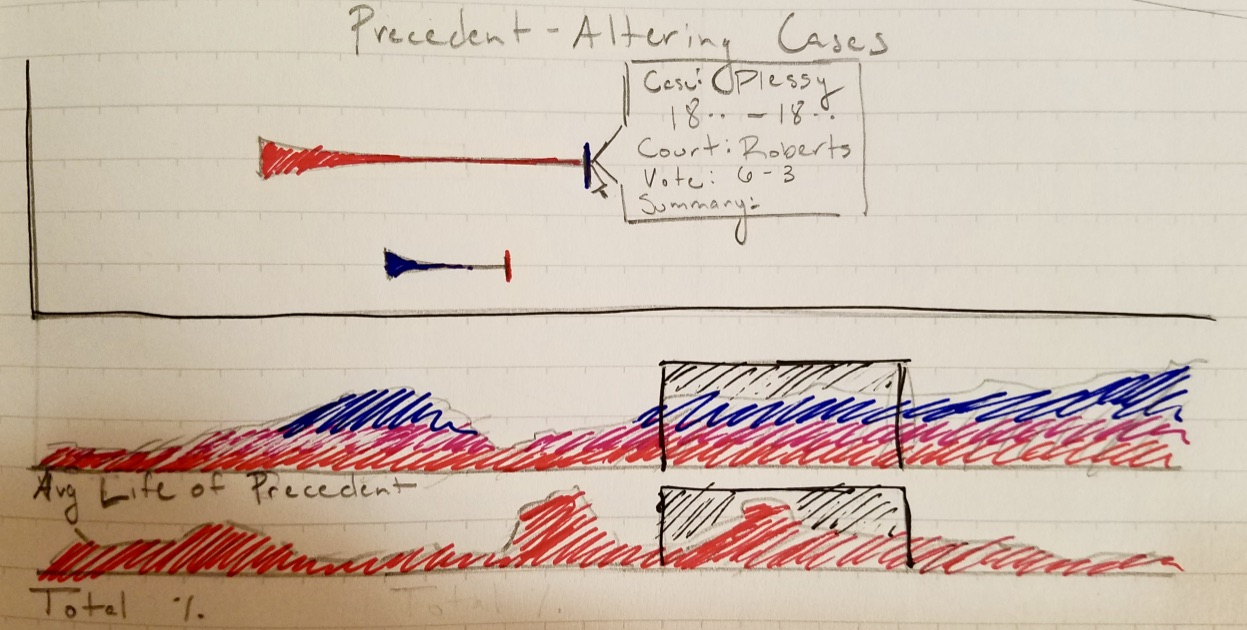
\includegraphics[width=\linewidth]{pics/precedentalteration.jpg}
    \caption{Precedent-Altering Rulings}
    \label{fig:roughprecedent}
\end{figure}
\FloatBarrier
The above visualization shows analysis of how precedent is altered over time.  Specifically, the funnel represents the start and end of a precedent-setting case that was eventually overturned by the Supreme Court.  The width of the funnel would change for each year to show how many times the original case was cited in that year.  The bar at the end of the funnel shows the Supreme Court case that overturned the original precedent.\\

The color of the funnel (and the bar) represent the ideological leaning of the original (or Supreme Court overruling) case.  We expect these to often be opposite colors, as rulings that overturn precedent often lean in the opposite ideological direction as the original ruling.\\

The top filled line chart represents the average life of a precedent set during a given year.  Upon further consideration, this was scrapped from the design, as we believe it can be potentially confusing without providing much insight into the Court.\\

The bottom filled line chart represents what percentage of cases that the Court views in a given year overturned a precedent.  This graph allows users to see a proxy of ``judicial activism," in which the Court uses its power to affect change to the existing policies set out by earlier courts.  This visualization would have a brush-and-zoom effect that could be used to control the upper chart.

\begin{figure}[h!]
    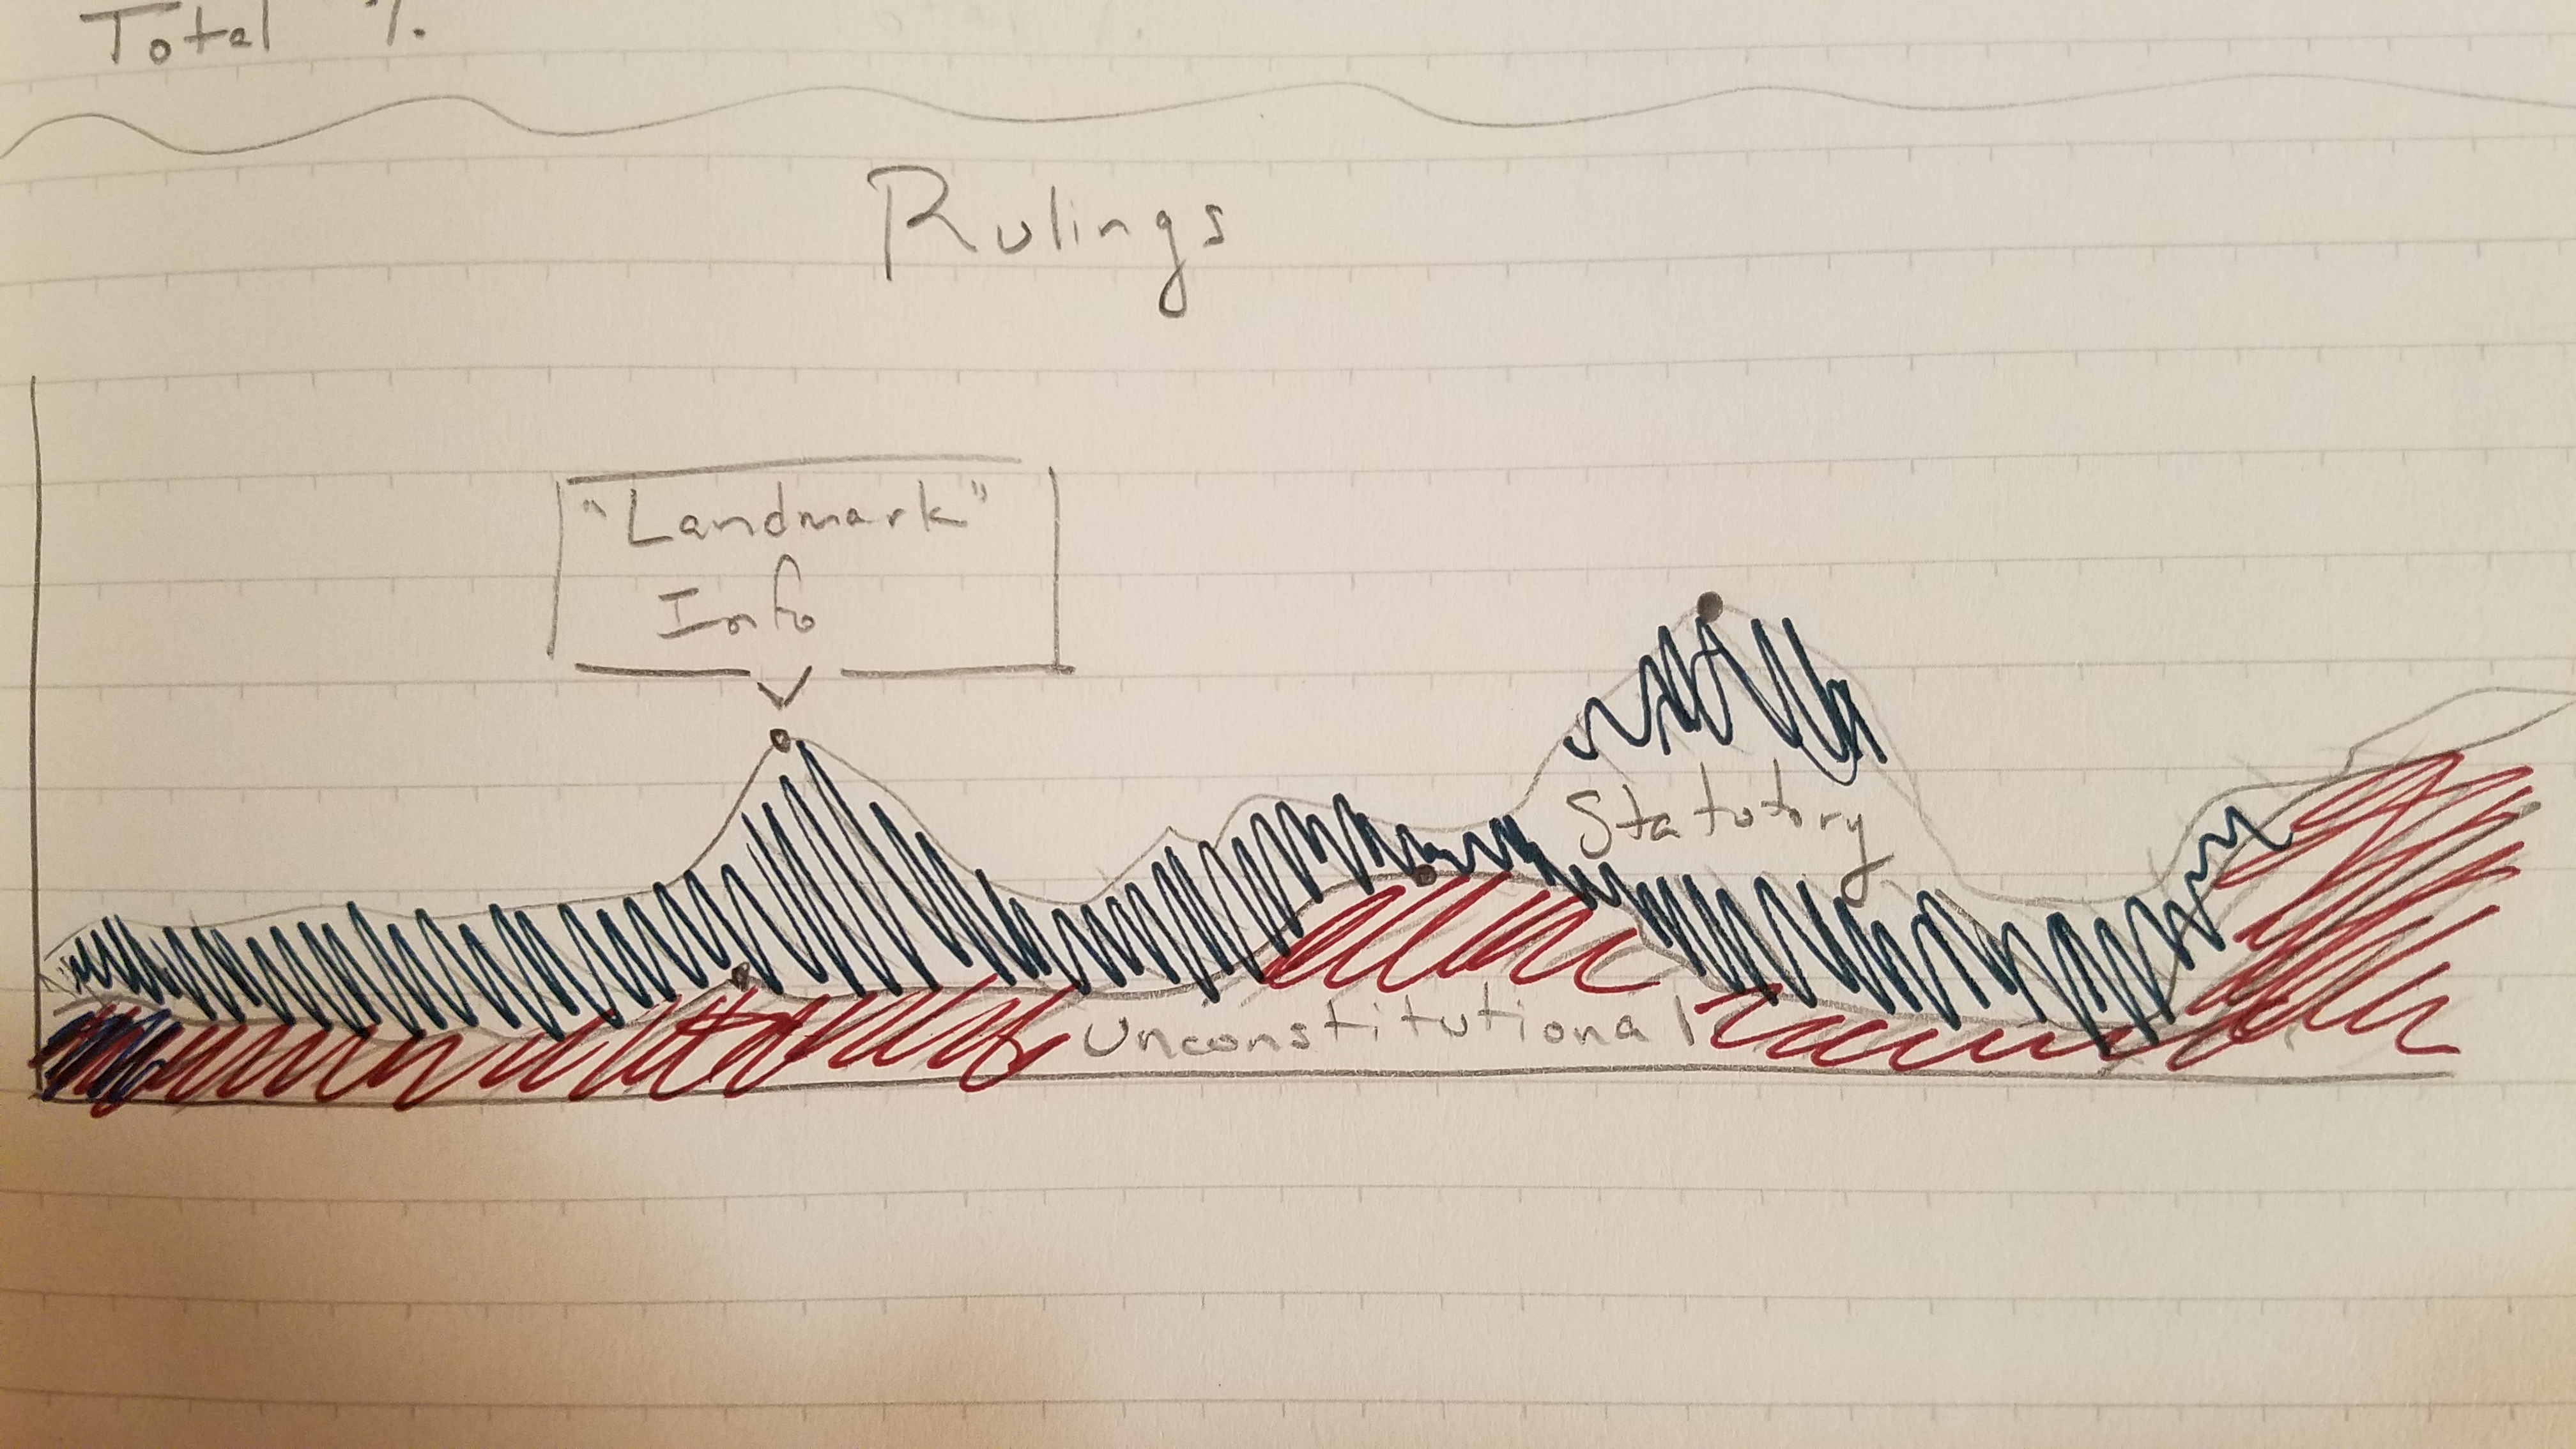
\includegraphics[width=\linewidth]{pics/Rulings.jpg}
    \caption{Rulings by Issue Area}
    \label{fig:roughrulings}
\end{figure}
\FloatBarrier
This sketch is a little more straightforward -- it simply shows the number of cases in a given year that the Court ruled unconstitutional, using a stacked line graph, with different colors for unconstitutional vs other types of rulings.  This allows users to get a sense of how the Court uses its power of judicial review.\\

In addition, landmark cases could be added as individual points, allowing users to explore how rulings that do not affect constitutional interpretation still have major affects on American policy.

\subsection{Option 2}
To represent the court’s ideology, we can aggregate the total number of cases according to the decision direction in a given period of time; this information would be linked to the ideological direction that each one of the justices had in their votes, the aggregation in this case will be showed with circles colored according ideology to which a gooey effect has been applied. A brush can be applied to the first visualization to filter a range of time, the individual justice’s votes will then show a more granulated view until the point where only cases decided on the same day are aggregated. Zooming the first general visualization will also be allowed.
\begin{figure}[h!]
  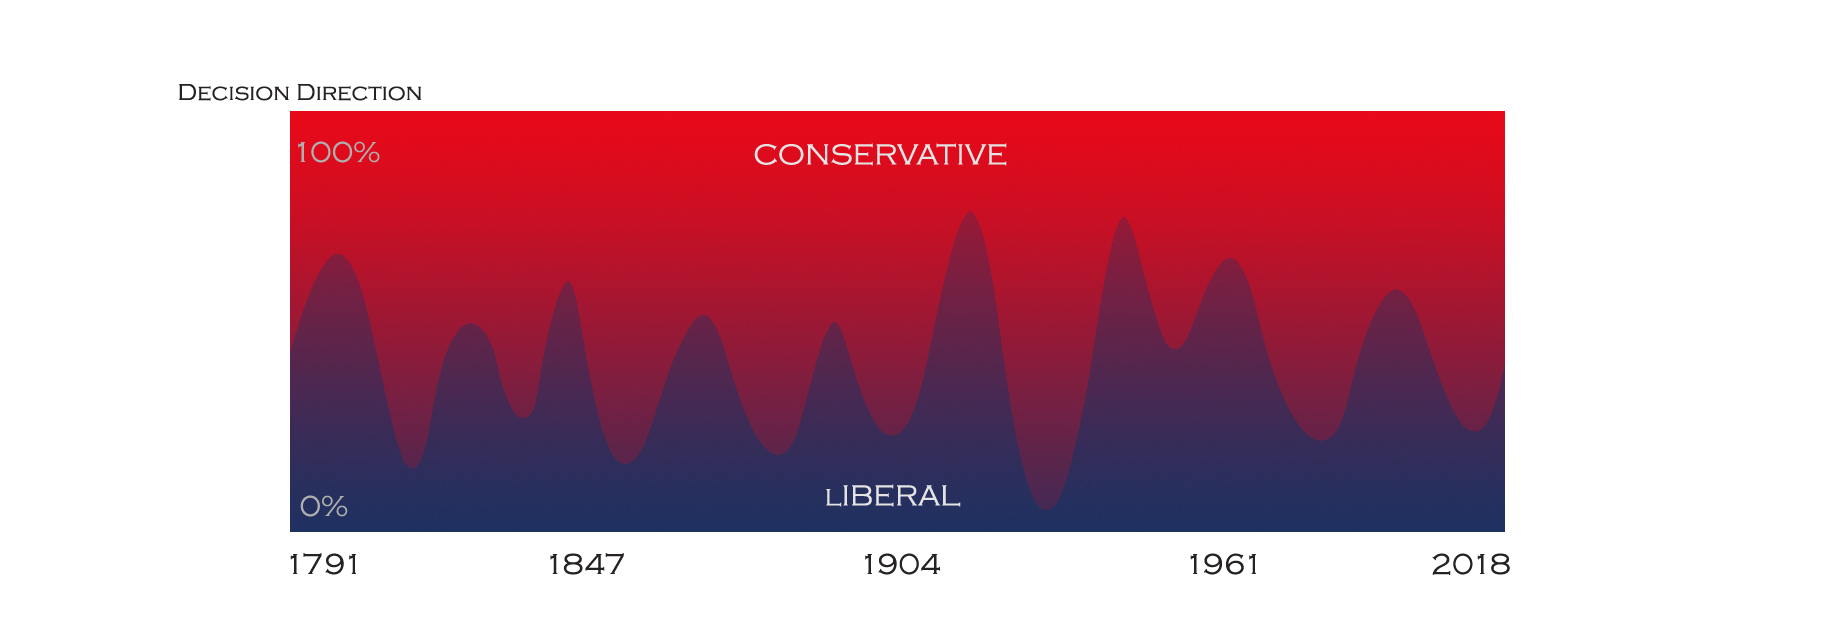
\includegraphics[width=\linewidth]{pics/ideologyCourt.jpg}
  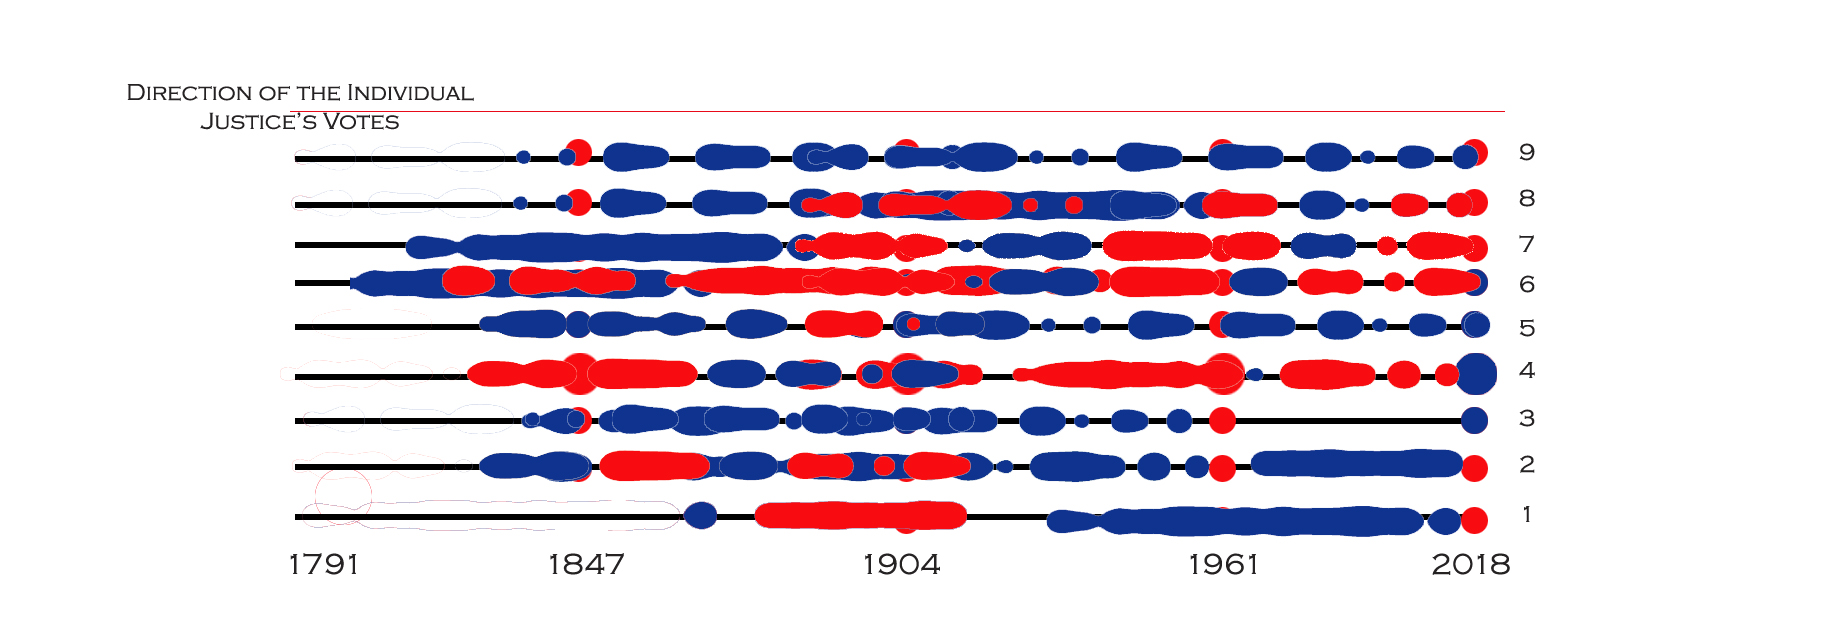
\includegraphics[width=\linewidth]{pics/ideologyJustices.jpg}
  \caption{Ideology}
  \label{fig:ideologyCourt}
\end{figure}
\FloatBarrier
The visualization for unconstitutional rulings will be presented as a stacked graph, where each layer represents an issue area. As we expect to have few unconstitutional cases, they will be shown directly over the respective layer as shown in Figure~\ref{fig:unconstitutionalRuling}:
\begin{figure}
    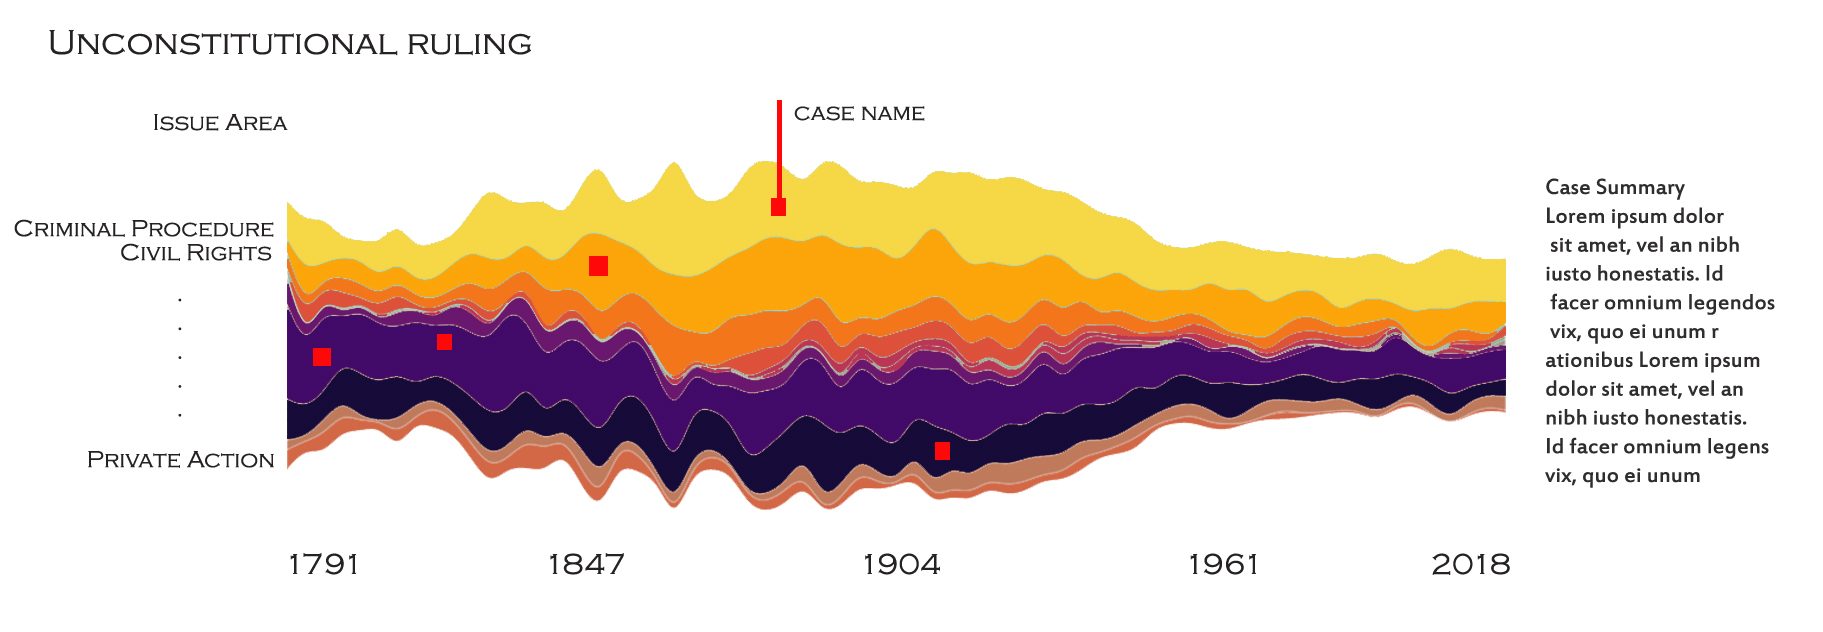
\includegraphics[width=\linewidth]{pics/unconstitutionalRuling.jpg}
    \label{fig:unconstitutionalRuling}
    \caption{Unconstitutional Ruling}
\end{figure}
\FloatBarrier
On hovering a mark representing a case with declaration of unconstitutionality, the name of the case will be shown as a tooltip as well as a brief summary. Since one of the objectives of this visualization is to analyze its correlation with society, some important landmarks occurred at that period of time will be shown below the visualization. Zooming is also allowed to have a more specific information about each issue area.
Finally, visualizing the precedence alteration will have a similar view, with highlighted marks representing cases that caused overturn of previous cases. Hovering a mark will show a tooltip with a summary of the case and clicking the mark will produce a graph showing all precedence cases in a timeline. In addition to the original objective, this visualization will show the validity time of a case.
\begin{figure}[h!]
  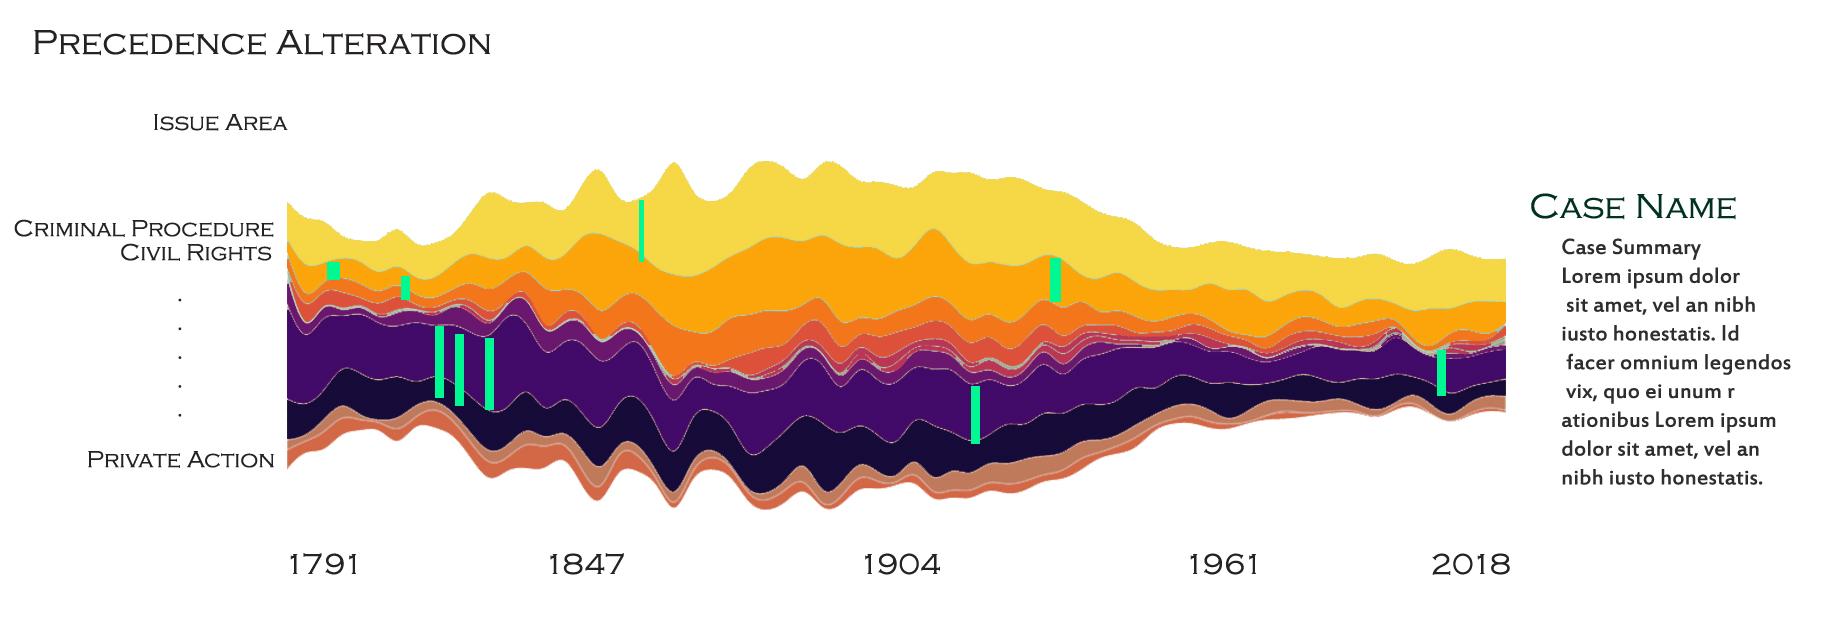
\includegraphics[width=\linewidth]{pics/precedenceAlteration.jpg}
  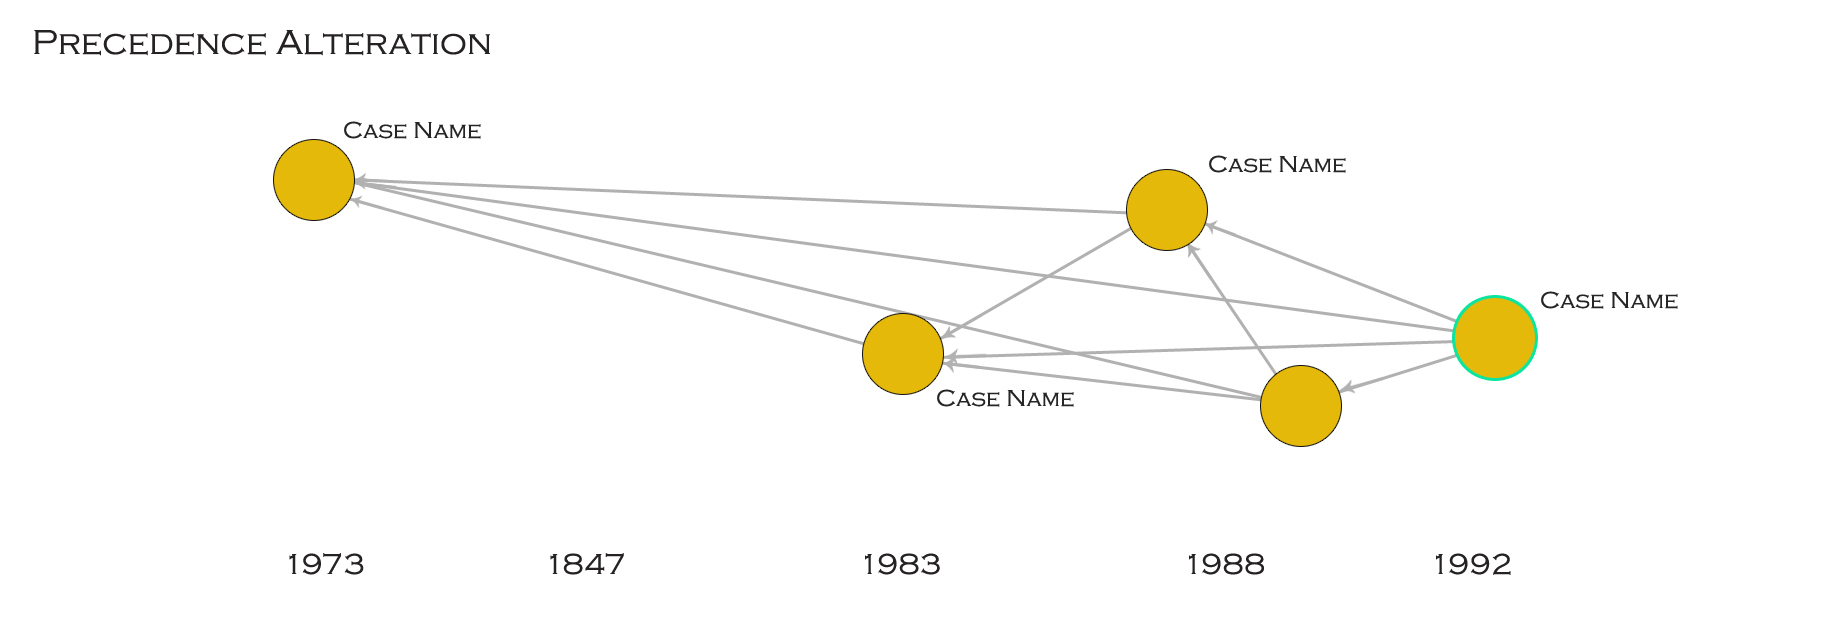
\includegraphics[width=\linewidth]{pics/precedenceAlteration1.jpg}
  \label{fig:ideologyCourt}
\end{figure}
\FloatBarrier

\subsection{Option 3}
For the third option of visualizing the data, the ideology data is represented as a combination of a bar chart and line graph. The bars would indicate in either direction the number of cases with rulings leaning that particular direction whereas the line would indicate the average position of judges. Brushing over this graph would alter the below visualizations.\\

The bottom left radar plot shows each of the issue areas discussed in the selected time frame via the above visualization. The blue line here indicates the percentage of cases discussing each issue area, and the red lines indicate the percentage of cases in that issue area that have an unconstitutional ruling.\\

The bottom right scatter-plot displays the number of cases in which precedent has been altered for a particular issue area encoded in the radius of the circles. Ideally this would show trends of how precedent changes as well as the frequency of precedent change over time in general. 
\begin{figure}[h!]
  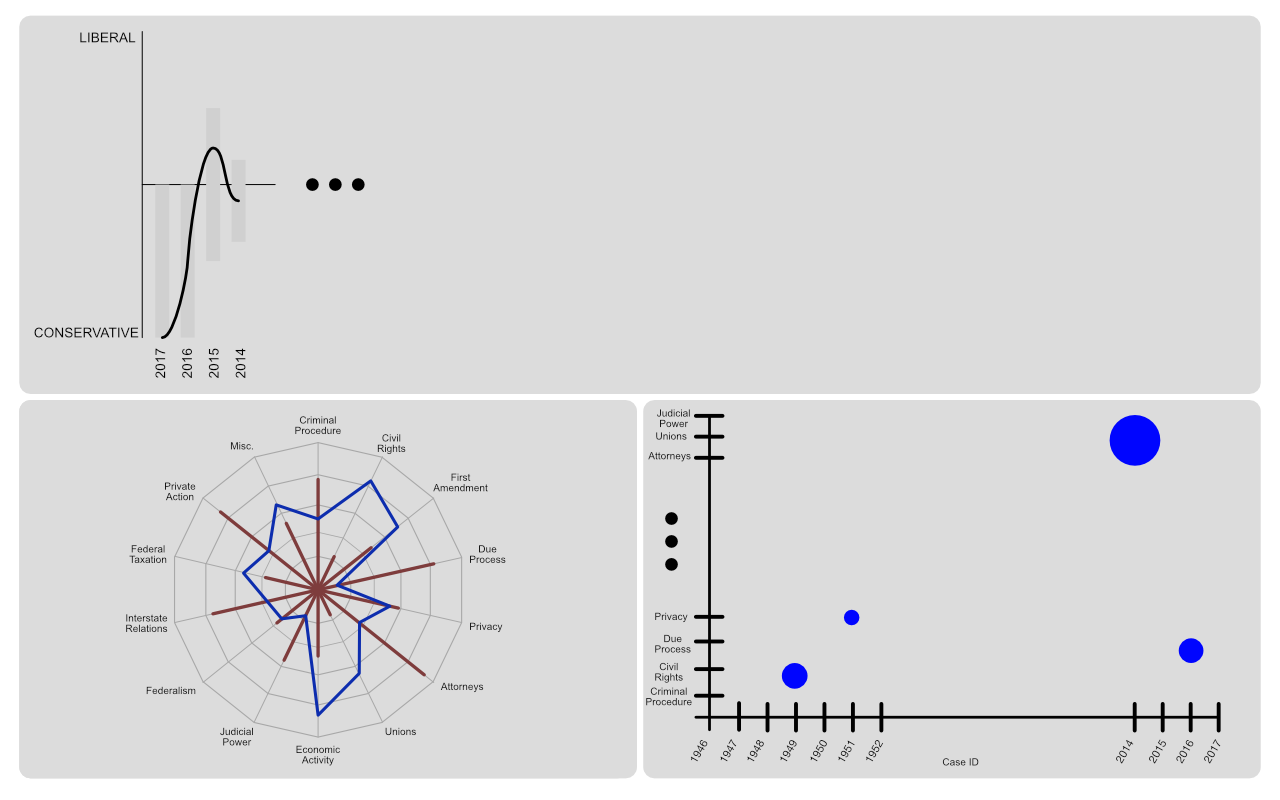
\includegraphics[width=\linewidth]{pics/Design3.png}
  \caption{Collective Visualization}
  \label{fig:collectiveVis}
\end{figure}
\FloatBarrier

\subsection{Final Design}
For the final design, the ideology data is represented as a combination of a bar chart and line graph. The bars would indicate in either direction the number of cases with rulings leaning that particular direction whereas the line would indicate the average position of judges. Brushing over this graph would alter the below visualizations. On hover over a bar, the number of cases ruled either liberal or conservative will display. In the top right corner a legend will be displayed informing the user of the the columns mean and what the line means. In the final visualization, the graph will extend all the way to the right to the year 2017.\\

The bottom left visualization shows the percentage of unconstitutional rulings per issue areas during the time selected in the main visualization (Ideology of the Supreme court). A legend in the bottom left will display the meaning of both the blue and red lines. On hovering each issue area, it will be highlighted and on clicking them the bottom right plot will filter the values accordingly.\\

The bottom right plot, which we will be calling a scatterwave plot, displays cases which alter precedent during the time span selected by brushing the top visualization.  Each wave on the plot represents one case that was overturned by the Supreme Court; the width of the wave for a given year is the number of times the original case was cited in that year.  The bars on the left and the right of the wave represent the original case (on the left) and the case that overturns it (on the right), and are color-encoded to show the ideological leaning of each ruling.  The waves themselves are color-coded by issue area.  Hovering over the wave will give information about the original case and the Supreme Court case that overruled it.
\begin{figure}[h!]
  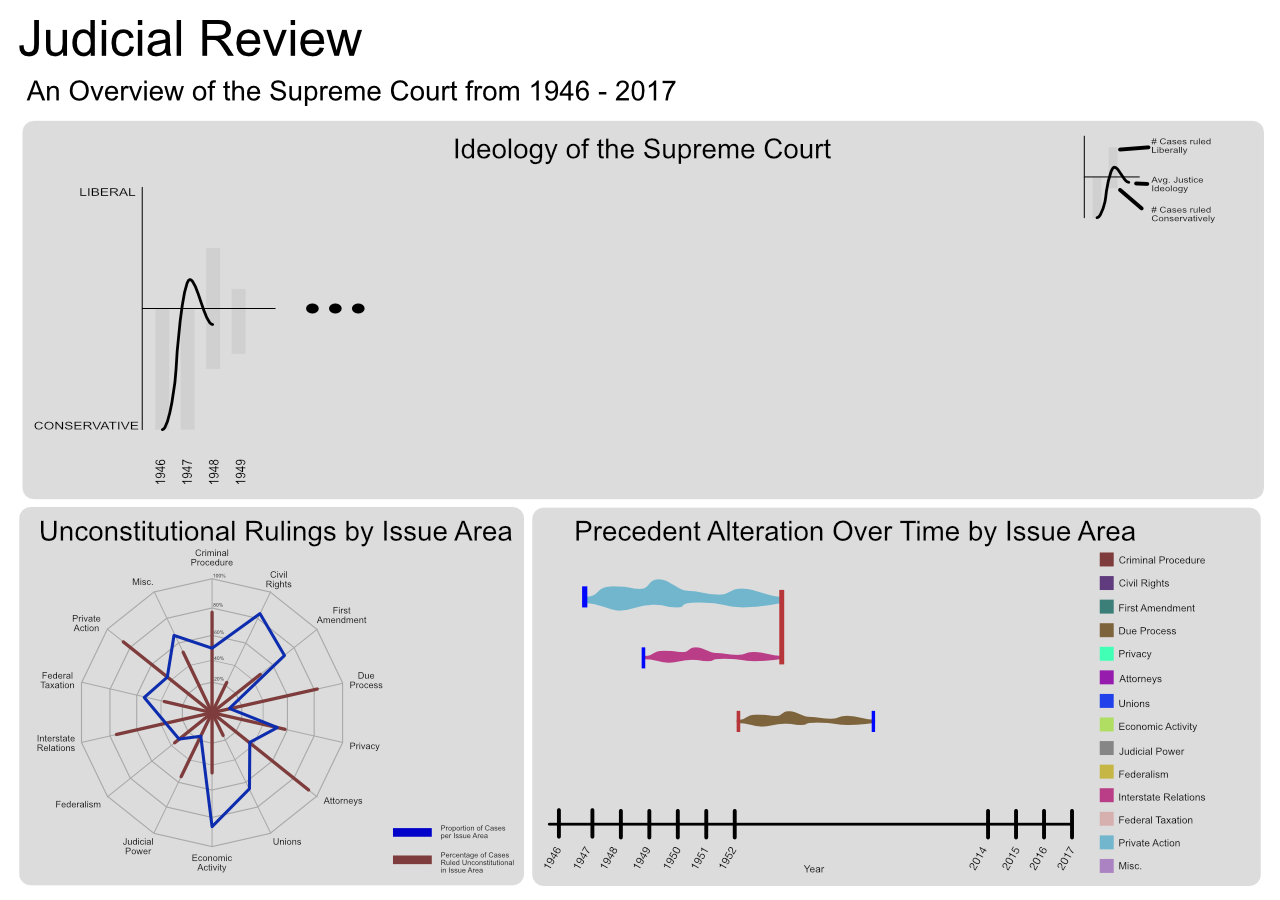
\includegraphics[width=\linewidth]{pics/FinalDesign.png}
  \caption{Final Design}
  \label{fig:finalVis}
\end{figure}
\FloatBarrier

\section{Must-Have Features}
Please see section 5.4.

\section{Optional Features}
We had a number of additional features that we thought could be included in our website; however, we are not sure if we could implement them in the time given.  One of these features is showing how the Court touches each section of American life by visualizing the origin of the court's cases, whether that be by subject area, geographical location, or litigant.  The major challenge for this features is figuring out how it would fit into the existing visualization.

Additionally, we believe the scatterwave plot is a relatively unique feature, and if we have extra time we considered packaging it as an official D3 package.

\section{Project Schedule}
The following Gantt chart shows our proposed project schedule.  While this will be adhered to throughout the process, we also plan on using an agile development approach to our work, including creating a backlog, story points, and a project board.  We believe this will keep us on track and efficient.  The Gantt chart also does not include anything about the process book, which should be kept up to date on a weekly basis.
\begin{figure}[h!]
\centering
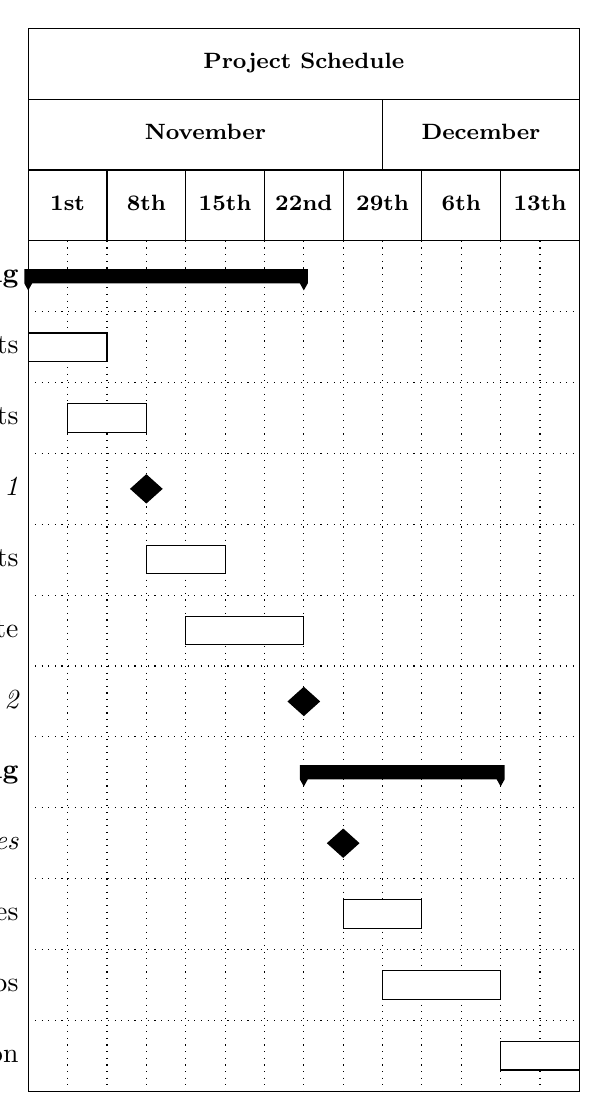
\begin{tikzpicture}
\begin{pgfinterruptboundingbox}
    \begin{ganttchart}[canvas/.append style={alias=frame}, x unit=0.5cm, y unit title=0.9cm, y unit chart=0.9cm, vgrid, hgrid, title height=1, title label font=\bfseries\footnotesize, group peaks width={0.2}]{1}{14}
    \gantttitle{Project Schedule}{14} \\
    \gantttitle[]{November}{9} 
    \gantttitle[]{December}{5} \\
    \gantttitle[]{1st}{2}
    \gantttitle[]{8th}{2}
    \gantttitle[]{15th}{2}
    \gantttitle[]{22nd}{2}
    \gantttitle[]{29th}{2}
    \gantttitle[]{6th}{2}
    \gantttitle[]{13th}{2} \\
    \ganttgroup{Prototyping}{1}{7} \\
    \ganttbar{Plan Objects}{1}{2} \\
    \ganttbar{Create Objects}{2}{3} \\
    \ganttmilestone{Milestone 1}{3} \\
    \ganttbar{Link Objects}{4}{5} \\
    \ganttbar{Bring Together Website}{5}{7} \\
    \ganttmilestone{Milestone 2}{7} \\
    \ganttgroup{Refining and Editing}{8}{12} \\
    \ganttmilestone{User Studies}{8} \\
    \ganttbar{Respond to User Studies}{9}{10} \\
    \ganttbar{Final Touch-Ups}{10}{12} \\
    \ganttbar{Finalize Presentation}{13}{14}
    \end{ganttchart}
\end{pgfinterruptboundingbox}
\useasboundingbox (frame.south west) rectangle (frame.north east);
\end{tikzpicture}
\end{figure}
\FloatBarrier

\printbibliography

\end{document}
